 \documentclass[a4paper,12pt]{report}

%Packages Used
\usepackage{amssymb,latexsym,amsmath}     % Standard packages
\usepackage{setspace}
\usepackage{sectsty}
\usepackage{titlesec}
\usepackage{hyperref}
\usepackage{bookmark}
\usepackage{graphics,graphicx}
\usepackage{tikz}
\usepackage{mathtools}
\usepackage{graphicx}
\usepackage{esvect}

\DeclarePairedDelimiter\abs{\lvert}{\rvert}%
\DeclarePairedDelimiter\norm{\lVert}{\rVert}%


\bookmarksetup{
  numbered,
  open
}
\renewcommand*{\thesection}{\arabic{section}}
\onehalfspacing

%Margins
\addtolength{\textwidth}{1.0in}
\addtolength{\textheight}{1.00in}
\addtolength{\evensidemargin}{-0.75in}
\addtolength{\oddsidemargin}{-0.75in}
\addtolength{\topmargin}{-.50in}

%%%%%%%%%%%%%%%%%%%%%%%%%%%%%% 
% Theorem/Proof Environments %
%%%%%%%%%%%%%%%%%%%%%%%%%%%%%%
\newtheorem{theorem}{Theorem}
\newenvironment{proof}{\noindent{\bf Proof:}}{$\hfill \Box$ \vspace{10pt}}
\sectionfont{\fontsize{12}{15}\selectfont}
\titlespacing*{\section}{0.5pt}{0.25\baselineskip}{0.25\baselineskip}

\begin{document}
\noindent
Yufei Lin

\noindent
Problem Set 2

\noindent
Sep \(17^{th}\) 2019

\begin{center}
\textbf{Problem Set 2}
\end{center}

\noindent
\textbf{Chapter 2}

\noindent
\textbf{1.(i)} $1^2+\dots+n^2=\frac{n(n+1)(2n+1)}{6}$.

\noindent
\textbf{Proof: }

\noindent
Let $n=1$, then we have on the left hand side:
\begin{align*}
1^2 = 1
\end{align*}

\noindent
Then, on the right hand side:
\begin{align*}
\frac{1\times (1+1)\times (2\cdot{1}+1)}{6} 
&= \frac{1\times 2\times 3}{6}\\
&=\frac{6}{6}\\
&=1
\end{align*}
\noindent
Therefore, left hand side equals to right hand side. This claim holds for 1.

\noindent
Then, assume if $n=k$, and $1^2+\dots+k^2=\frac{k(k+1)(2k+1)}{6}$.

Let $n=k+1$, on the left hand side, we would have:
\begin{align*}
1^2+\dots+k^2+(k+1)^2
&=\frac{k(k+1)(2k+1)}{6}+ (k+1)^2\\
&= \frac{k(k+1)(2k+1)}{6} + \frac{6(k+1)^2}{6}\\
&=\frac{k(k+1)(2k+1)}{6} + \frac{6(k+1)\cdot{(k+1)}}{6}\\
&=\frac{((k+1)(2k^2+k)+(6k+6)(k+1))}{6}\\
&=\frac{(k+1)(2k^2+k+6k+6)}{6}\\
&=\frac{(k+1)(2k^2+7k+6)}{6}\\
&=\frac{(k+1)(2k+3)(k+2)}{6}
\end{align*}
\begin{align*}
\phantom{1^2+\dots+k^2+(k+1)^2}
&=\frac{(k+1)(2(k+1)+1)((k+1)+1)}{6}\\
&=\frac{(k+1)((k+1)+1)(2(k+1)+1)}{6}\\
\end{align*}

\noindent
And on the right hand side, we would have:
\[\frac{(k+1)((k+1)+1)(2(k+1)+1)}{6}\]
\[\therefore \text{Left hand side equals to right hand side}\]
The claim holds. 

\noindent
\textbf{1.(ii)} $1^3+\dots+n^3=(1+\dots+n)^2$.

\noindent
\textbf{Proof: }

\noindent
Let $n=1$, then we would have on the left hand side:
\[1^3=1\]

\noindent
On the right hand side:
\[1^2=1\]

\noindent
Therefore, left hand side equals to right hand side this claim holds for 1.

\noindent
Then, assume if $n=k$, and $1^3+\dots+k^3=(1+\dots+k)^2$.

\noindent
Let $n=k+1$, on the left hand side, we would have:
\begin{align*}
1^3+\dots+k^3+(k+1)^3
&=(1+\dots+k)^2+(k+1)^3\\
&=(\frac{k(k+1)}{2})^2+(k+1)^3\\
&=(\frac{k^2(k+1)^2}{4})+(k+1)\cdot{(k+1)^2}\\
&=\frac{k^2}{4}\cdot{(k+1)^2}+(k+1)\cdot{(k+1)^2}\\
&=(k+1)^2\cdot{(\frac{k^2}{4}+(k+1))}\\
&=(k+1)^2\cdot{(\frac{k^2}{4}+\frac{4(k+1)}{4})}\\
&=(k+1)^2\cdot{(\frac{k^2}{4}+\frac{4k+4}{4})}\\
\end{align*}
\begin{align*}
\phantom{1^3+\dots+k^3+(k+1)^3}
&=(k+1)^2\cdot{(\frac{k^2+4k+4}{4}}\\
&=(k+1)^2\cdot{(\frac{(k+2)^2}{4}}\\
&=(k+1)^2\cdot{(\frac{(k+2)}{2})^2}\\
&=(k+1)^2\cdot{(\frac{((k+1)+1)}{2})^2}\\
&=(\frac{(k+1)((k+1)+1)}{2})^2\\
&=(1+\dots+(k+1))^2
\end{align*}

\noindent
And on the right hand side, we would have:
\[(1+\dots+(k+1))^2\]
\[\therefore \text{Left hand side equals to right hand side}\]
The claim holds. 

\noindent
\textbf{2.(i)}$$\sum_{i=1}^{n} (2i-1)=n^2$$

\noindent
\textbf{2.(ii)}

\begin{align*}
\sum_{i=1}^{n} (2i-1)^2
&=\sum_{i=1}^{2n} (i)^2-\sum_{i=1}^{n} (2i)^2\\
&=\sum_{i=1}^{2n} (i)^2-4\sum_{i=1}^{n} (i)^2\\
&=\frac{(2n)((2n)+1)(2(2n)+1)}{6}\\
&=\frac{(2n)(2n+1)(4n+1)-4n(n+1)(2n+1)}{6}\\
&=\frac{(2n)(2n+1)(4n+1-2n-2)}{6}\\
&=\frac{(2n)(2n+1)(2n-1)}{6}
\end{align*}

\noindent
\textbf{3.(a)}

\noindent
On the right hand side we have:
\begin{align*}
\binom n{k-1}+\binom nk
&=\frac{n!}{(k-1)!(n-(k-1))!}+\frac{n!}{k!(n-k)!}\\
&=\frac{k\cdot{n!}+(n-k+1)\cdot{n!}}{k!(n-k+1))!}\\
&=\frac{(k+n-k+1)n!}{k!((n+1)-k))!}\\
&=\frac{(n+1)!}{k!((n+1)-k))!}\\
&=\binom {n+1}{k}
\end{align*}
\[\therefore \text{Left hand side is the same as the right hand side.}\]

\noindent
\textbf{3.(b)}

\noindent
$\forall n, n \in \mathbb{Z}_{\geq 0}$,we would have by definition \(\binom nn=\binom n0=1\), which is a natural number. 

\noindent
Let $n=0$, we would have \(\binom 00=1\), and it is a natural number. The claim holds for 0. 

\noindent
Then, assume $n=m$ and \(\forall k, k\leq m, \binom mk\) is natural number.

\noindent
Let $n=m+1$, we would have \(\forall k, k<m+1, \binom {m+1}k=\binom m{k-1}+\binom m{k}\) from the theorem we prove in (a). It is because from the assumption above, we have both \(\binom m{k-1},\binom m{k}\) are natural numbers. Therefore, \(\binom {m+1}k\) is a natural number. And \(\binom {m+1}{m+1}={m+1}0=1\) by definition of a binomial coefficient. Therefore, the claim holds for all $n \in \mathbb{Z}_{\geq 0}$.

\noindent
\textbf{3.(c)}

\noindent
When choosing $k$ things out of $n$ things, we are looking at the arrangement of first $k$ things in an ordered list of $n$ things without considering their order. THerefore, first we are arranging all $n$ things, then we have $n!$ ways to do the arrangment. Then, we choose the first $k$ things and find their arrangements. Therefore, we are overcounting all such arrangements by $(n-k)!$times, since we do not care about the rest $n-k$ things' arrangements. Then we would have $\frac{n!}{(n-k)!}$ ways of arrangement left. However, we are still overcounting the arrangements $k!$ times because we do not need to know the order fo the arrangements of these $k$ things. Therefore, we have $\frac{n!}{k!\cdot{(n-k)}!}$ in total.

\noindent
\textbf{3.(d)}

\noindent
Let $n=1$, then we have on the left hand side: $(a+b)^1=a+b$ and on the right hand side: \(\binom 10 a^1+\binom 11b^1=a+b\). We have left hand side equals to the right hand side. The claim holds for $n=1$. 

\noindent
Let $n=m$, such that $(a+b)^m=a^m+\binom m1a^{m-1}b+\binom m2a^{m-2}b^2+\dots+\binom m{m-1}ab^{m-1}+b^m$ 

\noindent
Let $n=m+1$, on the left hand side we would have:
\begin{align*}
(a+b)^{m+1}
&=(a+b)^m\cdot{(a+b)}\\
&=(a^m+\binom m1a^{m-1}b+\binom m2a^{m-2}b^2+\dots+\binom m{m-1}ab^{m-1}+b^m)\cdot{(a+b)}\\
&=a\cdot{\left(\binom m0 a^m+\binom m1a^{m-1}b+\binom m2a^{m-2}b^2+\dots+\binom m{m-1}ab^{m-1}+\binom mm b^m\right)}\\
&\qquad+b\cdot{\left(\binom m0 a^m+\binom m1a^{m-1}b+\binom m2a^{m-2}b^2+\dots+\binom m{m-1}ab^{m-1}+\binom mm b^m\right)}\\
&=\binom m0 a^{m+1}+\binom m1a^mb+\dots+\binom m{m-1} a^2b^{m-1} + \binom mm ab^m\\
&\qquad+\binom m0 a^mb +\binom m1 a^mb^2+\dots+\binom m{m-1} ab^m+\binom mm b^{m+1}\\
&=\binom m0 a^{m+1}+\left(\binom m0+\binom m1\right)a^mb+\dots+\left(\binom m{m-1}+\binom mm\right)ab^m+\binom mm b^{m+1}\\
\end{align*}
It's because from (a) we have proved that \(\binom n{k-1}+\binom nk=\binom {n+1}k\).Also, by definition of a binomial coefficient we know that \(\forall m, m\in \mathbb{Z}_{\geq0} \binom m0=\binom mm=1\) Therefore, on the left hand side, we should have:
\begin{align*}
&\qquad\binom m0 a^{m+1}+\left(\binom m0+\binom m1\right)a^mb+\dots+\left(\binom m{m-1}+\binom mm\right)ab^m+\binom mm b^{m+1}\\
&=\binom {m+1}0 a^{m+1}+\binom {m+1} a^mb+\dots+\binom {m+1}m ab^m+b^{m+1}\\
&=\sum_{j=0}^{m+1} \binom {m+1}j a^{m+1-j}b^j
\end{align*}
On the right hand side, we would have when $n=m+1$:$$\sum_{j=0}^{m+1} \binom {m+1}j a^{m+1-j}b^j$$
\[\therefore \text{Left hand side equals to the right hand side. The claim holds.}\]

\noindent
\textbf{3.(e)}

\textbf{(i)}

\noindent
\textbf{Proof:}

\noindent
Let $n=0$, then we would have on the left hand side \(\binom 00=1\), and on the right hand side, we would have $2^0=1$. Therefore, the claim holds for $n=0$. 

\noindent
Let $n=m$ such that $$\sum_{j=0}^{m} \binom {m}j=2^m$$

\noindent
Let $n=m+1$, we would have on the left hand side:
\begin{align*}
\sum_{j=0}^{m+1} \binom {m+1}j
&=\binom {m+1}0+\binom {m+1}1+\dots+\binom {m+1}{m+1}\\
&=\binom m0+\left(\binom m0+\binom m1\right)+\dots+\left(\binom m{m-1}+\binom mm\right)+\binom {m}{m}\\
&=\binom m0+\binom m0+\binom m1+\binom m1+\dots+\binom {m}{m}+\binom {m}{m}\\
&=2\cdot{\left(\binom m0+\binom m1+\dots+\binom {m}{m}\right)}\\
&=2\cdot{2^n}\\
&=2^{n+1}
\end{align*}

\noindent
On the right hand side, we would have $2^{m+1}$. Thus, the left hand side is equal to the right hand side. The claim holds. \\

\textbf{(ii)}

\noindent
\textbf{Proof: }

\noindent
This only holds for any number $n, n> 0$. It is because if $n=0$, this equation would be 1 instead of 0. 

\noindent
Let $n=1$, on the left hand side we would have \(\binom 10-\binom 11 = 0\). On the right hand side we have $0$. Therefore, the claim holds for $n=1$.

\noindent
Let $n=m$, assume $$\sum_{j=0}^{m} (-1)^j\cdot{\binom {m}j}=0$$

\noindent
Let $n=m+1$, we would have on the left hand side:
\begin{align*}
\sum_{j=0}^{m+1} (-1)^j\cdot{\binom {m+1}j} 
&= \binom {m+1}0 - \binom {m+1}1 +\dots +(-1)^{m+1}\cdot{\binom {m+1}{m+1}}\\
&= \binom {m}0 - \left(\binom {m}0+\binom {m}1\right) +\dots +(-1)^{m}\cdot{\left(\binom m{m-1}+\binom mm\right)}+(-1)^{m}\cdot{\binom mm}\\
&=\binom {m}0-\binom {m}0-\binom {m}1+\dots+(-1)^{m}\cdot{\binom m{m-1}}+(-1)^{m}\cdot{\binom mm}+(-1)^{m}\cdot{\binom mm}\\
&=0
\end{align*}
On the left hand side, we have $0$.

\noindent
Therefore, this claim holds for all number $n>0$.\\

\textbf{(iii) and (iv)}

\noindent
\textbf{Proof:}

\noindent
From the question above we have proved that $\sum_{j=0}^{m} (-1)^j\cdot{\binom {m}j}=0$. This means that for even binomial coefficients, it is always posivtive in this equation, and for odd coefficients, it is always negative. Therefore, we can have $\sum_{j \text{ even}} \binom {n}j=\sum_{j \text { odd}} \binom {n}j$. It is because from (i) we know $\sum_{j=0}^{m} \binom {m}j=2^n$. Thus, $\sum_{j \text{ even}} \binom {n}j=\sum_{j \text { odd}} \binom {n}j=2^{n-1}$

\noindent
\textbf{5.(a)}

\noindent
Let $n=0$, we would have on the left hand side: $r^0=1$.

\noindent
On the right hand side, we would have:
\begin{align*}
\frac{1-r^{0+1}}{1-r}
&=\frac{1-r}{1-r}\\
&=1\\
\end{align*}
\[\therefore \text{Left hand side is the same as the right hand side.}\]
The claim holds for $n=0$.

\noindent
Let $n=k$, assume $1+\dots+r^k=\frac{1-r^{k+1}}{1-r}$

\noindent
If $n=k+1$, then on the left hand side we would have:
\begin{align*}
1+\dots+r^k+r^{k+1}
&=\frac{1-r^{k+1}}{1-r}+r^{k+1}\\
&=\frac{1-r^{k+1}}{1-r}+\frac{(1-r)r^{k+1}}{1-r}\\
&=\frac{1-r^{k+1}}{1-r}+\frac{r^{k+1}-r^{k+2}}{1-r}\\
&=\frac{1-r^{k+1}+r^{k+1}-r^{k+2}}{1-r}\\
&=\frac{1-r^{k+2}}{1-r}\\
&=\frac{1-r^{(k+1)+1}}{1-r}
\end{align*}
On the right hand side, we have:
$\frac{1-r^{(k+1)+1}}{1-r}$.
\[\therefore \text{Left hand side is the same as the right hand side.}\]
The claim holds.

\noindent
\textbf{5.(b)}

\noindent
Let $S=1+\dots+r^n$, by multiplying both sides with $r$, then we would have:
\begin{align*}
r\cdot{S}
&=r\cdot{1+\dots+r^n}\\
&=r+\dots+r^{n+1}\\
\end{align*}
It is because we would like to know about $S$, then we could have:
\begin{align*}
r\cdot{S}-S
&=(r-1)\cdot{S}\\
&=r+\dots+r^{n+1}-(1+\dots+r^n)\\
&=r^{n+1}-1
\end{align*}
\[\therefore(r-1)\cdot{S}=r^{n+1}-1\]
\[S=\frac{r^{n+1}-1}{r-1}=\frac{1-r^{n+1}}{1-r}\]

\pagebreak
\noindent
\textbf{Chapter 3}

\noindent
\textbf{1.(i)}
\begin{align*}
f(f(x))
&=f(\frac{1}{1+x})\\
&=\frac{1}{1+\frac{1}{1+x}}\\
&=\frac{1}{\frac{2+x}{1+x}}\\
&=\frac{1+x}{2+x}
\end{align*}
\[\therefore x\neq -1,-2\]

\noindent
\textbf{1.(ii)}

\begin{align*}
f(\frac{1}{x})
&=\frac{1}{1+\frac{1}{x}}\\
&=\frac{1}{\frac{1+x}{x}}\\
&=\frac{x}{1+x}
\end{align*}
\[\therefore x\neq -1\]

\noindent
\textbf{1.(iii)}
\begin{align*}
f(cx)
&=\frac{1}{1+cx}
\end{align*}
\[\therefore x\neq -\frac{1}{c}, if c\neq 0\]

\noindent
\textbf{1.(iv)}
\begin{align*}
f(x+y)
&=\frac{1}{1+x+y}
\end{align*}
\[\therefore x+y\neq -1\]

\noindent
\textbf{1.(v)}
\begin{align*}
f(x)+f(y)
&=\frac{1}{1+x}+\frac{1}{1+y}\\
&=\frac{2+x+y}{(1+x)(1+y)}
\end{align*}
\[\therefore x,y\neq -1\]

\noindent
\textbf{1.(vi)}

\noindent
$f(cx)=f(x), x\neq -1, or -c^{-1}$, then we would have $\frac{1}{1+x}=\frac{1}{1+cx}$.
\[\therefore 1+x=1+cx\]
\[(c-1)x=0\]
If we only want one $x$ solution for such an equation, then we could have $(c-1)\cdot{0}=0$. Therefore, $c\in \mathbb{R}$ the equation would always hold. 

\noindent
\textbf{1.(vii)}

\noindent
If we would like to have at least two different answers for $x$ in the equation $(c-1)x=0$, then we need to have $c-1=0$. Thus, $c=1$. 

\noindent
\textbf{2.(i)}

\noindent
It is because for any $y$ is rational, $h(y)= 0$, and for any $y$ that is irrational, $h(y)=1$. If we would like to have $h(y)\geq y$, then we need $y\leq0, y\in \mathbb{Q}$ or $y<1, y \in \mathbb{R-Q}$.

\noindent
\textbf{2.(ii)}

\noindent
It's because we want to have $h(y)\leq g(y)$. Thus meaning for $y\in \mathbb{Q}$, $y^2\geq 0$, and for $y \in \mathbb{R-Q}, y^2\geq 1$. Therefore, $|y|\geq 0,y\in \mathbb{Q}$ or $|y|>1,y \in \mathbb{R-Q}$

\noindent
\textbf{2.(iii)}

\noindent
Suppose $z$ is a rational number, then we have $h(z)=0$, and $h(g(z))=0^2=0$. Therefore, $h(g(z))-h(z)=0$.
Suppose $z$ is a irrational number, we would have $h(z)=1$, and $h(g(z)) = 1^2=1$. Therefore,  $h(g(z))-h(z)=0$.
In conclusion, $h(g(z))-h(z)=0$. 

\noindent
\textbf{2.(iv)}

\noindent
For $g(w)\leq w$, we would have $w-w^2=w\cdot{(1-w)}\geq 0$. Thus, $w$ and $1-w$ should be the same sign or one of them is $0$. 

\noindent
Both of them are positive:
\begin{align*}
w> 0\\
1-w> 0
\end{align*}
Therefore, $1>w>0$.

\noindent
Both of the are negative:
\begin{align*}
w< 0\\
1-w< 0
\end{align*}
This is not possible, because we need $w>1$ and $w<0$.

\noindent
If one of them is $0$. Say $w$, then $w=0$. If$w-1=0$, then $w=1$.

\[\therefore 1\geq w\geq 0\]

\noindent
\textbf{2.(v)}

\noindent
Suppose $g(g(e))=g(e)$, then we have $g(e^2)=e^4=e^2$. Then we have:
\begin{align*}
e^4-e^2=0\\
e^2\cdot{(e^2-1)}=0\\
e^2=0 \text{ or } e^2-1 = 0\\
e_1=0 \text{ and } e_{2,3}=\pm 1
\end{align*}

\noindent
\textbf{3.(i)}

\noindent
$1-x^2\geq 0$. Thus, $1\geq x^2$. Therefore, $-1\leq x\leq 1$.

\noindent
\textbf{3.(ii)}

\noindent
$1-\sqrt{1-x^2}\geq 0$, and we know $1+\sqrt{1-x^2}$. Thus, we can have:
\begin{align*}
(1-\sqrt{1-x^2})\cdot{1+\sqrt{1-x^2}}&\geq(1+\sqrt{1-x^2})\cdot{0}\\
1-1+x^2&\geq 0\\
x^2&\geq 0
\end{align*} 
\[\therefore x\in \mathbb{R}\]

\noindent
\textbf{3.(iii)}

\noindent
$x\neq1,2$

\noindent
\textbf{3.(iv)}

\noindent
$1-x^2\geq 0$ and $x^2-1\geq 0$. Thus, we have $1\geq x^2 and 1\leq x^2$. Therefore, $x^2=1$ and $x_{1,2}=\pm 1$. 

\noindent
\textbf{3.(v)}

\noindent
$1-x\geq 0, x-2\geq 0$. Therefore, $1\geq x$ and $x\leq 2$ It is not possible. Therefore, this function cannot happen in real number domain. 

\noindent
\textbf{4.(i)}

\noindent
We should have the following:
\begin{align*}
(S\circ P)(y)
&=S(P(y))\\
&=S(2^y)\\
&=(2^y)^2\\
&=2^{2y}
\end{align*}

\noindent
\textbf{4.(ii)}

\noindent
We should have the following:
\begin{align*}
(S\circ s)(y)
&=S(P(y))\\
&=S(sin(y))\\
&=(sin(y))^2\\
&=sin^2(y)
\end{align*}

\noindent
\textbf{4.(iii)}

\noindent
We should have the following:
\begin{align*}
(S\circ P\circ s)(t)+(s\circ P)(t)
&=S(P(s(t)))+s(P(t))\\
&=S(P(sin(t))) + s(2^t)\\
&=S(2^{sin(t)})+sin(2^t)\\
&=(2^{sin(t)})^2+sin(2^t)
\end{align*}

\noindent
\textbf{4.(iv)}

\noindent
We should have the following:
\begin{align*}
s(t^3)
&=sin(t^3)
\end{align*}

\noindent
\textbf{5.}

\noindent
$S(x)=x^2,P(x)=2^x,s(x)=sinx$

\noindent
\textbf{5.(i)}

\noindent
We should have the following:
\begin{align*}
f(x)&=2^{sinx}
&=2^(s(x))\\
&=P(s(x))\\
&=(P\circ s)(x)
\end{align*}

\noindent
\textbf{5.(ii)}

\noindent
We should have the following:
\begin{align*}
f(x)&=sin(2^x)\\
&=sin(P(x))\\
&=s(P(x))\\
&=(s\circ P)(x)
\end{align*}

\noindent
\textbf{5.(iii)}

\noindent
We should have the following:
\begin{align*}
f(x)&=sin(x^2)\\
&=sin(S(x))\\
&=s(S(x))\\
&=(s\circ S)(x)
\end{align*}

\noindent
\textbf{5.(iv)}

\noindent
We should have the following:
\begin{align*}
f(x)&=sin^2(x)\\
&=(sin(x))^2\\
&=(s(x))^2\\
&=S(s(x))\\
&=(S\circ s)(x)
\end{align*}

\noindent
\textbf{5.(v)}

\noindent
We should have the following:
\begin{align*}
f(t)&=2^{2^t}\\
&=2^{P(t)}\\
&=P(P(t))\\
&=(P\circ P)(x)
\end{align*}

\pagebreak
\noindent
\textbf{5.(vi)}

\noindent
We should have the following:
\begin{align*}
f(u)&=sin(2^u+2^{u^2})\\
&=sin(P(u)+2^S(u))\\
&=sin(P(u)+P(S(u)))\\
&=s(P(u)+(P\circ S)(u))\\
&=s(P+P\circ S)(u)
\end{align*}

\noindent
\textbf{5.(vii)}

\noindent
We should have the following:
\begin{align*}
f(y)&=sin(sin(sin(2^{2^{sin y}})))\\
&=sin(sin(sin(2^{2^{s(y)}})))\\
&=sin(sin(sin(2^{P(s(y))})))\\
&=sin(sin(sin(P(P(s(y))))))\\
&=s(s(s(P(P(s(y))))))\\
&=(s\circ s\circ s\circ P\circ P\circ s)(y)
\end{align*}

\noindent
\textbf{5.(viii)}

\noindent
We should have the following:
\begin{align*}
f(a)&=2^{sin^2(a)}+sin(a^2)+2^{sin(a^2+sin(a))}\\
&=2^{s(a)^2}+sin(S(a))+2^{sin(S(a)+s(a))}\\
&=2^{S(s(a))}+s(S(a))+2^{s(S(a)+s(a))}\\
&=P(S(s(a)))+s(S(a))+P(s(S(a)+s(a)))\\
&=P(S(s(a)))+s(S(a))+P(s(S(a)+s(a)))\\
&=(P\circ S\circ s)(a)+(s\circ S)(a)+(P\circ s(S+s))(a)
\end{align*}

\noindent
\textbf{21.(a)}

\noindent
This is not equivalent. Let $f(x)=x^2$ and $g(x)=x,h(x)=1$. Thus, $f\circ (g+h)(x)=f(x+1)=(x+1)^2=x^2+2x+1$ and $f\circ g(x)+f\circ h(x)=f(x)+f(1)=x^2+1^2=x^2+1$. Therefore, they are not the same. 

\noindent
\textbf{21.(b)}
We know that for any two given functions $a(x)+b(x)=(a+b)(x)$. Therefore, in this equatiion, we have on the left hand side:
\begin{align*}
((g+h)\circ f)(x)
&=(g+h)(f(x))\\
&=g(f(x))+h(f(x))\\
&=(g\circ f)(x)+(h\circ f)(x)\\
&=RHS
\end{align*}

\noindent
\textbf{21.(c)}

\noindent
Let $h(x)=1/x$, then on the left hand side, we would have $1/(f\circ g)=(h\circ (f\circ g))(x)$. On the right hand side, we would have $(1/f)\circ g=((h\circ f)\circ g)(x)$. From the theroerm stating that composition of functions are associative, we know that $(h\circ (f\circ g))(x)=((h\circ f)\circ g)(x)$. Thus, LHS=RHS. 

\noindent
\textbf{21.(d)}

\noindent
This is not equivalent. For instance, let $f(x)=2, g(x) =x$. Then, on the left hand side we would have $\frac{1}{(f\circ g)(x)}=\frac{1}{f(x)}=\frac{1}{2}$. On the right hand side, we would have $(f\circ \frac{1}{g})(x)=f(1/x)=2$. Therefore, left hand side does not equal to right hand side. 

\noindent
\textbf{22.(a)}

\noindent
It is because $g(x)=(h\circ f)(x)=h(f(x))$, we would have $g(x)=h(f(x))$ and $g(y)=h(f(y))$. If $f(x)=f(y)$, then $h(f(x))=h(f(y))\rightarrow g(x)=g(y)$. Therefore, if $f(x)=f(y)$, then $g(x)=g(y)$.

\noindent
\textbf{22.(b)}

\noindent
Suppose whenever $f(x)=f(y)$, $g(x)=g(y)$. Let $h(z)$ be a function that takes in $z=f(x)$. If $f(x)=f(y)$, we would have $h(f(x))=h(f(y))$ because we know if the values of the variable is the same then the value of the function is the same. We also know that $g(x)=g(y)$, then we can say that $g(x)=h(f(x))=g(y)=h(f(y))$. Thus, $g(x)=(h\circ f)(x)$. 

\noindent
\textbf{23.(a)}

\noindent
Want to prove that if $x\neq y$, then $g(x)\neq g(y)$. Thus, showing if $g(x)=g(y)$, then $x=y$ still holds. Thus, suppose $g(x)=g(y)$, we would have $f(g(x))=f(g(y))=I(x)=I(y)=x=y$. Therefore, $x=y$.

\noindent
\textbf{23. (b)}

\noindent
Suppose $b=f(a)$, and let $a=g(x)$. From the identity function we know that all $f(g(x))=x$, meaning for all $a=g(x)$ we can have $b=f(a)=f(g(x))=x$. Also, because the domain of $I=x$ is all real numbers. Therefore, for any number $b$ there exist an $a$ such that $b=f(a)$.

\pagebreak
\noindent
\textbf{Chapter 4}

\noindent
\textbf{1.(i)}

\noindent
$2<x<4$

\begin{figure}[h]
  \centering
  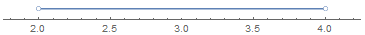
\includegraphics[width=10cm]{Pics/Chap41(i).png}
  \caption{1.(i)}
\end{figure}

\noindent
\textbf{1.(ii)}

\noindent
$2\leq x\leq4$

\begin{figure}[h]
  \centering
  
\includegraphics[width=10cm]{./Pics/Chap41(ii).png}
  \caption{1.(ii)}
\end{figure}

\noindent
\textbf{1.(iii)}

\noindent
For $\epsilon \geq 0$, we have $a-\epsilon \leq x \leq a+\epsilon$

\noindent
For $\epsilon < 0$, the inequality does not hold. 

\begin{figure}[h]
  \centering
  
\includegraphics[width=10cm]{Pics/Chap41(iii).png}
  \caption{1.(iii)}
\end{figure}

\pagebreak
\noindent
\textbf{1.(iv)}

\noindent
$-\frac{\sqrt{6}}{2}<x<-\frac{\sqrt{2}}{2}\cup \frac{\sqrt{2}}{2}<x<\frac{\sqrt{6}}{2}$ 

\begin{figure}[h]
  \centering
  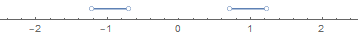
\includegraphics[width=10cm]{Pics/Chap41(iv).png}
  \caption{1.(iv)}
\end{figure}

\noindent
\textbf{1.(v)}

\noindent
$-2\leq x\leq 2$ 

\begin{figure}[h]
  \centering
  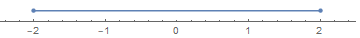
\includegraphics[width=10cm]{Pics/Chap41(v).png}
  \caption{1.(v)}
\end{figure}

\pagebreak
\noindent
\textbf{1.(vi)}

\noindent
For $1\leq a$, we have $x\in \mathbb{R}$

\begin{figure}[h]
  \centering
  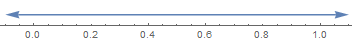
\includegraphics[width=10cm]{Pics/Chap41(vi)1.png}
  \caption{1.(vi)2}
\end{figure}

\noindent
For $1\geq a \geq 0$, we have $-\sqrt{1-a} \geq x \cup x\geq \sqrt{1-a}$

\begin{figure}[h]
  \centering
  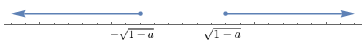
\includegraphics[width=10cm]{Pics/Chap41(vi)2.png}
  \caption{1.(vi)2}
\end{figure}

\noindent
For $a < 0$, the inequality does not hold.\\ 

\noindent
\textbf{1.(vii)}

\noindent
$-1\geq x\cup x\geq 1$ 

\begin{figure}[h]
  \centering
  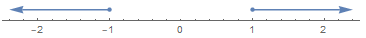
\includegraphics[width=10cm]{Pics/Chap41(vii).png}
  \caption{1.(vii)}
\end{figure}

\pagebreak
\noindent
\textbf{1.(viii)}

\noindent
$-1< x<1\cup x>2$ 

\begin{figure}[h]
  \centering
  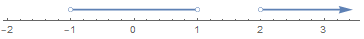
\includegraphics[width=10cm]{Pics/Chap41(viii).png}
  \caption{1.(viii)}
\end{figure}

\noindent
\textbf{11.}

\begin{enumerate}
\item[(i)] f(-x)=f(x). Thus, it is symmetry according to y-axis.
\item[(ii)] f(-x)=-f(x). Thus, this function is symmetry according to origin.
\item[(iii)] It has no parts touching the third or fourth quadrant.
\item[(iv)] $f(x)=f(x+a)$ would repeat itself every $a$ intervals, like $sin(x)$.
\end{enumerate}














\end{document}